\documentclass[a4paper]{scrartcl}
\usepackage[landscape]{geometry}
\usepackage[skip=3ex]{parskip}
\usepackage{amsmath}
\usepackage[utf8]{inputenc}
\usepackage{./tikz-uml}
\usepackage{fancyhdr}
\usepackage{float}
\usepackage{titling}

\usetikzlibrary{positioning}

\pagestyle{fancy}
\fancyhf{}
\lhead{\theauthor\quad-\quad\thetitle}
\rhead{\thepage}
\rfoot{}

\newcommand{\eq}{\,\ensuremath{=}\,}
\newcommand{\gt}{\,\ensuremath{>}\,}
\newcommand{\lt}{\,\ensuremath{<}\,}
\newcommand{\xo}{\,\ensuremath{\mid}\,} 

\let\oldle\le\renewcommand{\le}{\,\ensuremath{\oldle}\,}
\let\oldge\ge\renewcommand{\ge}{\,\ensuremath{\oldge}\,}

\newenvironment{umldiag}
{\begin{center}\begin{tikzpicture}}
{\end{tikzpicture}\end{center}}

\title{Travel to the Moon}
\author{Gruppo 73}
\date{March 2024}
\begin{document}
	
%%%%%%%%%%%%%%%%%%%%%%%%%%%%%%%%%%%%%%%%%%%%%%%%%%%%%%%%%%%%%%%%%%%%%%%%%%%%%%%%
\newpage\section{Raffinamento dei Requisiti}\vskip2em
%%%%%%%%%%%%%%%%%%%%%%%%%%%%%%%%%%%%%%%%%%%%%%%%%%%%%%%%%%%%%%%%%%%%%%%%%%%%%%%%

%\subsection{A}
%\begin{enumerate}
%	\item blah bleh
%\end{enumerate}
\subsection{Requisiti sulle crociere}
\begin{enumerate}
    \item \textbf{Codice}: ??
    \item \textbf{Data di inizio}: Data
    \item \textbf{Data di fine}: Data
    \item \textbf{Nave utilizzata} (vedi Req. 2)
    \item \textbf{Itinerario} (vedi Req. 3)
    \item \textbf{Tipo}:
    \begin{enumerate}
        \item \textbf{Luna di miele}, di cui interessa:
        \begin{enumerate}
            \item \textbf{Sottotipo}:
            \begin{enumerate}
                \item Tradizionale
                \item Alternative
            \end{enumerate}
        \end{enumerate}
        \item \textbf{Per famiglie}:
        \begin{enumerate}
            \item Adatta ai bambini (bool)
        \end{enumerate}
    \end{enumerate}
\end{enumerate}

\subsection{Requisiti della Nave}
\begin{enumerate}
    \item \textbf{Nome}: string
    \item \textbf{Confort}: 3..5
    \item \textbf{Capienza}: int > 1
\end{enumerate}

\subsection{Requisiti sugli itinerari}
Di ogni itinerario mi interessa:
\begin{enumerate}
    \item Sequenza ordinata di elementi, per ogni uno:
    \begin{enumerate}
        \item \textbf{Nome}: string
        \item \textbf{Destinazioni ordinate} (vedi Req. 4)
        \item \textbf{Data di arrivo} (relativa alla partenza iniziale):
        \begin{enumerate}
            \item Numero giorno
            \item Ora
        \end{enumerate}
        \item \textbf{Data di ripartenza} (relativa alla partenza iniziale):
        \begin{enumerate}
            \item Numero giorno
            \item Ora
        \end{enumerate}
    \end{enumerate}
\end{enumerate}

\subsection{Requisiti sulle destinazioni}
\begin{enumerate}
    \item \textbf{Nome}: string
    \item \textbf{Continente}: ??
    \item \textbf{Posti da vedere} (vedi Req. 5)
    \item \textbf{Tipo}, almeno uno tra:
    \begin{enumerate}
        \item Romantico
        \item Divertente
    \end{enumerate}
\end{enumerate}

\subsection{Requisiti sui posti da vedere}
\begin{enumerate}
    \item \textbf{Nome}
    \item \textbf{Descrizione}
    \item \textbf{Orari di appertura}, nella forma di una mappa che associa ad ogni giorno della settimana un insieme di fascie orarie dove ogni fascia oraria è definita come una coppia di orari
\end{enumerate}

\subsection{Requisiti cliente}
\begin{enumerate}
    \item \textbf{Nome}: string
    \item \textbf{Cognome}: string
    \item \textbf{Data di nascita}: Data
    \item \textbf{Indirizzo}: Indirizzo
\end{enumerate}

\subsection{Requisiti prenotazione}
\begin{enumerate}
    \item \textbf{Istante}: DataOra
    \item \textbf{Numero posti prenotati}: int > 0
\end{enumerate}



%%%%%%%%%%%%%%%%%%%%%%%%%%%%%%%%%%%%%%%%%%%%%%%%%%%%%%%%%%%%%%%%%%%%%%%%%%%%%%%%
\newpage\section{Diagramma delle Classi}\vskip2em
%%%%%%%%%%%%%%%%%%%%%%%%%%%%%%%%%%%%%%%%%%%%%%%%%%%%%%%%%%%%%%%%%%%%%%%%%%%%%%%%
\begin{figure}[H]
    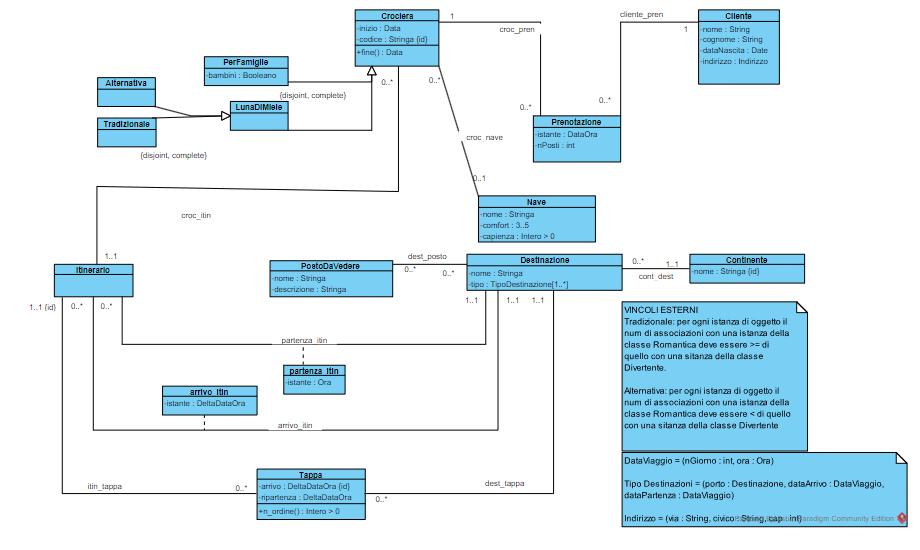
\includegraphics[width=1\linewidth]{../export.png}
\end{figure}
% \begin{umldiag}
% 	% \umlclass[below left = 5cm of A]{B}{}{}
% 	% \umlCNinherit[stereo=complete disjoint]{A}{x,y}{B}
% 	% \umlassoc[arg1=1..*|a, arg2=1..1|b, anchors=150 and 30]{A}{B}	
% \end{umldiag}

%%%%%%%%%%%%%%%%%%%%%%%%%%%%%%%%%%%%%%%%%%%%%%%%%%%%%%%%%%%%%%%%%%%%%%%%%%%%%%%%
\newpage\section{Dizionario dei Dati}\vskip2em
%%%%%%%%%%%%%%%%%%%%%%%%%%%%%%%%%%%%%%%%%%%%%%%%%%%%%%%%%%%%%%%%%%%%%%%%%%%%%%%%

%\begin{enumerate}
%	\item
%\end{enumerate}

\begin{itemize}
    \item TipoDestinazione = \{romantica, divertente\}
    \item Indirizzo = (via: string, civico: string, cap: Cap)
    \item Cap = (d1: 0..9, d2: 0..9, d3: 0..9, d4: 0..9, d5: 0..9)
    \item DeltaDataOra = (giorno: Intero > 0, orario: Ora)
\end{itemize}

\subsection{Operazioni sui tipi dato}
\begin{itemize}
    \item {Operazioni del tipo di dato "DeltaDataOra":}
    
    \textbf{<} (x:DeltaDataOra, y:DeltaDataOra) : Boolano
    
    \textbf{Precondizioni:} nessuna
    
    \textbf{Postcondizioni:} 
    $result = \text{true}$ se e solo se $(x.giorno < y.giorno)$ oppure $(x.giorno = y.giorno$ e $x.orario < y.orario)$
\end{itemize}

%%%%%%%%%%%%%%%%%%%%%%%%%%%%%%%%%%%%%%%%%%%%%%%%%%%%%%%%%%%%%%%%%%%%%%%%%%%%%%%%
\end{document}
